\subsection{Cumulative Voting\label{app:CV}}

CV is a prioritization method for prioritizing a list of items \cite{Leffingwell1999} and has been studied and applied in various fields.

In forestry it is used to take into account opinions of different parts of society while planning forest harvesting \cite{Laukkanen2004}.
CV has also been used as a voting mechanism in government elections \cite{Cooper2010} and to aid decision making in corporate governance \cite{Bhagat1984}. In computer science we have seen CV being part of various software algorithms, e.g.\ in \cite{Hoover2003} it is used as part of pattern detection algorithm that is used to locate the optic nerve in a retinal image.

In software engineering CV has been applied not only in requirements engineering and software release planning \cite{Heikkila2010}
but also in software security \cite{Baca2010}, software quality \cite{Barney2009b}, software metrics \cite{Berander2006}, software process improvement \cite{Pettersson2008}, and software verification and validation \cite{Feldt2010}.

Studies have also used CV as part of a research method itself. For instance, in \cite{Svahnberg2008} software impact analysis issues are elicited in structured interviews and afterwards the importance of each issue is determined with the help of CV. Whether CV has been used in a particular domain or as part of a methodology is in itself quite irrelevant as long as one takes into account the type of data CV results consist of.

CV has many synonyms in literature: hundred (100) dollar (\$) method\slash test and hundred (100) point method.
%Before being applied in software engineering CV was used for
%political elections \cite{Engstrom1999} and corporate governance \cite{Bhagat1984}. 
%CV has also been applied in e.g.\ decision making in forestry \cite{Hiltunen2008}, voting in social 
%networks \cite{Boldi:2009:VSN:1645953.1646052} and in computer algorithms for consensus 
%clustering \cite{Ayad2008b} (as a method for combining the results of different clustering algorithms).

In CV a stakeholder is given 100 points,
imaginary dollars or units of percentages that can be spent on the prioritization
items. In the simplest case, the stakeholder can spend any amount of points on any number
of items as long as the total amount adds up to 100. The more points
assigned to an item, the higher the priority of the item (and implicitly, 
the lower priority to the other items). 
The stakeholder may spend all points on just one item or distribute
them among all or some of the items. Once again, this is the simplest case; 
other variants exist, which we will see next.

Often prioritization is done by more than one stakeholder. The final
priority of an item can be calculated by adding up the points each stakeholder
has spent on it. Sometimes the vote of some stakeholders may be more
important than the votes of others. For example, a manager may be
more influential or shareholders may have different
amount of shares. In such a case the priorities of each stakeholder
may be multiplied by an individual coefficient or a stakeholder may be given a 
more points to perform the prioritization.

Worth mentioning in this context is that it is advisable to randomize 
the order of items in a prioritization list. This is necessary in order 
to minimize the effect of order on the prioritization
results, which has shown to have an effect \cite{Svahnberg2009}.

\subsubsection{Benefits and Drawbacks of Cumulative Voting}
Compared to analytical hierarchy process (AHP), CV is faster and easier to 
learn and use \cite{Berander2005,Ahl2005}.
AHP benefits from consistency check, but CV does not require this because
all prioritization items are evaluated simultaneously \cite{Ahl2005}.

There are, however, a few problems with CV. First of all, it cannot be repeated for the
same stakeholders and prioritization items due to stakeholder bias
\cite{Leffingwell1999} (c.f.\ Section~\ref{hcv}). Secondly, CV 
becomes more difficult to use when the number of prioritization items 
increases \cite{Berander2009a}.

\subsubsection{Example of Cumulative Voting with Several Stakeholders}

Let us next give an example of CV with several stakeholders. Suppose Robin,
Alice, and John are three friends who want to buy some beverages in
a store. They have different preferences but do not want to buy too
many drinks. Therefore, they decide to use CV to decide what to buy.
Each of the friends distributes 100 points between four items: milk,
tea, coffee, and juice (Step 1 in Figure~\ref{fig:Example-of-Cumulative}).
In this case each of them will spend a different amount of money on the purchase,
hence, their priorities are multiplied by different coefficients
(Step 2 and the stakeholder importance coefficient in Figure~\ref{fig:Example-of-Cumulative}).
The final beverage priorities are calculated by summing up the weighted priorities
of stakeholders (Step 3 in Figure~\ref{fig:Example-of-Cumulative}).

\begin{figure}
	\center
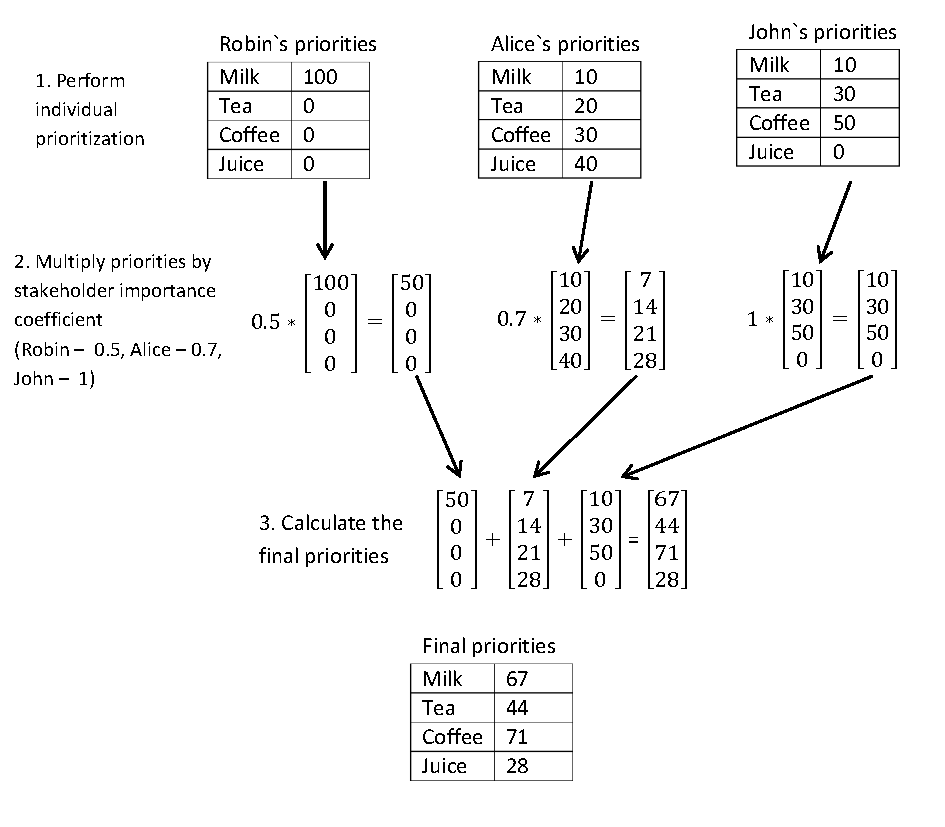
\includegraphics[scale=0.55]{fig/cv}
\caption{\label{fig:Example-of-Cumulative}Example of CV with several stakeholders.}
\end{figure}

\subsubsection{Stakeholder Bias\label{sub:Stakeholder-Bias}}

Prioritization using CV may be biased if a stakeholder knows the preferences
of other stakeholders. She may manipulate the results by spending more
points on items that are important to her but not to the other stakeholders.
On the one hand, stakeholder bias makes it unreasonable to repeat CV
with the same prioritization items and stakeholders. On the other hand,
this property of CV may be useful in giving more power to important
minority stakeholders, such as security experts or software testers.
Suppose the same software requirements are prioritized for a second time using
CV. A developer might know that all vital functionality is selected by
other stakeholders, but his toy feature is left out. In effect, the developer
could spend all his points on this feature to put it in the next release. 

Stakeholder bias may be mitigated by setting a maximum priority that
can be assigned to an item. This way each stakeholder is forced to
distribute the money between several prioritization items \cite{Berander2006a}.

Another bias is that people in general tend to assign round priority
values. This is likely caused by lack of objective judgement criteria. Either
way it seems to be a problem not acknowledged by many since all prioritization is largely
based on expert opinion.

\subsubsection{Scalability of Cumulative Voting---Hierarchical Cumulative Voting\label{hcv}}

The standard CV approach has a low scalability. If the number of prioritization items
is high, stakeholders may lose sight of the bigger picture and assign priorities to a
limited number of items. One, unsophisticated, solution to the problem is to provide
more points for prioritization (1,000 or 10,000 instead of 100); however, one could take another approach. 

When the number of prioritization items is high they can usually 
be grouped hierarchically by forming a tree structure (Figure~\ref{fig:Prionitization-Item-Hierarchy}) 
and, thus, parent-child dependencies will exist between many items.

\begin{figure}
	\center
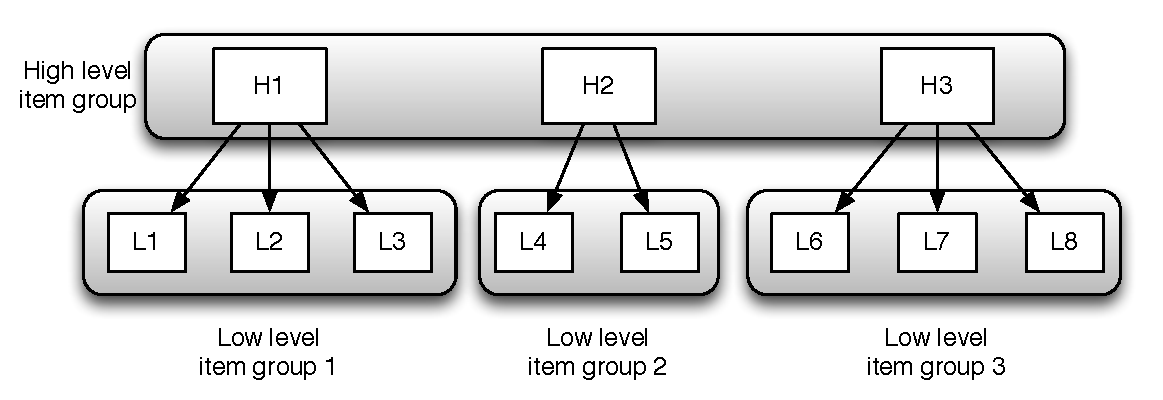
\includegraphics[scale=0.45]{fig/hcv-example1}
\caption{\label{fig:Prionitization-Item-Hierarchy}Example of prioritization item hierarchy.}
\end{figure}

In \cite{Berander2006a} the authors propose a method for prioritizing hierarchically
structured items called Hierarchical Cumulative Voting (HCV). It may
be seen as combination of the hierarchical part of the Analytical Hierarchy
Process (AHP) \cite{Berander2005,Saaty1980a} and the CV prioritization method.
Since items are prioritized in smaller sets, stakeholders do not lose
sight of the bigger picture during prioritization, and the prioritization of a large number
of requirements is considered easier.

\subsubsection{Compensation Factors\label{sub:Compensation-factor}}
HCV deals with the problem of prioritization scalability but it comes
at a cost. Low level item groups may consist of different numbers of
items, but the number of points spent on each group is the same, i.e.\ in
a small-sized group, the same amount of points is distributed among fewer items.
Hence, items in smaller groups are statistically more likely to have a higher priority, on 
average, compared to items in larger groups. To balance this difference each low
level prioritization item can be multiplied by a compensation factor \cite{Berander2006a}.

As an example, suppose an item ($A$) in a
group of 10 items is assigned 60 points. Hence, $A$ will receive 600
compensated points. In this case it is impossible for any item in
a group smaller than 6 items to compete with $A$. Even if item ($B$) in
a group of 5 is assigned the maximum number of points (100), the maximum compensated
priority value $B$ can receive is 500.

In \cite{Berander2009a} the authors suggest that compensated prioritization is more favorable
compared to uncompensated. But neither compensated nor uncompensated prioritization
is perfect and, as a general rule, it is better to keep the size of
prioritization item groups similar.

\subsubsection{HCV Execution}
According to \cite{Berander2006a}, HCV is conducted with the following
steps (Steps 4--5 are optional):

\begin{enumerate}
\item Construct hierarchy. Prioritization items need to be divided into
one high and several low level item groups. Each low level item group
is child to exactly one high level item. And each high level item
has one low level item group. One low level item may belong to several
item groups. Even if parts of the items are not logically connected they
can be grouped separately and assigned a fake parent item, e.g.\ `misc.
items'. HCV does not, as far as we know, provide any instructions for 
creating a requirements hierarchy.

\item Each high and low level item group is prioritized separately using
CV. The stakeholder may prioritize all item groups at once or one by one.
But it should be possible to prioritize groups in any order and repeatedly,
because the stakeholder might learn more about the items while performing the prioritization.

In particular the stakeholder is likely to learn more about a high level item when
prioritizing its low level item group \cite{Berander2009a}. Some stakeholders
may prioritize only part of the groups and each group may be prioritized
by different stakeholders.

\item The priority of each low level item is normalized by dividing it with
the sum of all low level priorities of each item in all groups.

%\begin{equation}
%p{}_{i\, normalized}=\frac{p_{i}}{\sum_{j=0}^{n}p_{j}}\label{eq:norm}
%\end{equation}

\item The final priority of each low level item is calculated by multiplying
it with the priority of its parent high level item.

\item Then one applies the compensation factor to all low level requirements as described
in Section~\ref{sub:Compensation-factor}.

\item Finally, when multiple stakeholders have performed the prioritization, priorities
of low level items are combined as in standard CV.
\end{enumerate}

It is possible that one low level item is child of more than one high
level requirement and, thus, belongs to two or more low level requirement
groups (see Figure~\ref{fig:Overlapping-Prioritization-Item}). Such
requirements participate in the standard HCV prioritization process and
are prioritized two or more times with each group they belong to.
At the end of the prioritization they receive several priority values.
These values can be summed together to form the final priority of the item.
(This is done because the item adds value to both parts of the hierarchy.)

\begin{figure}
	\center
\includegraphics[scale=0.5]{\string"fig/hcv hierarchy\string".png}
\caption{\label{fig:Overlapping-Prioritization-Item}Overlapping prioritization item hierarchy example.}
\end{figure}

\subsubsection{Example of Hierarchical Cumulative Voting}
Suppose six requirements
for a mobile phone operating system need to be prioritized: `reminder
alarm', `specify repeated event', `hide contact', `add picture to phonebook',
`search contact', `make video call'. Three high level requirements can
be identified: `Calendar', `Phonebook', `Call'. The low level requirements are then
grouped as sub-requirements of high level requirements as shown in
Figure~\ref{fig:Example-of-Hierachical}. The `Search contact' requirement is a 
sub-requirement and has two parent requirements:`Phonebook'
and `Call'. The computation of the final priorities of requirements is shown
in Table~\ref{tab:Example-of-Hierarchical}.

After requirements are grouped, and a hierarchy is defined, each group
of requirements are then prioritized using CV. The final priority of a low level
requirement is computed by multiplying the priority of the requirement
with the priority of its parent high level requirement and the compensation
factor. The compensation factor in this particular case is the number of elements
in a group, two for the `calendar' and `call' sub-requirements and three for
the `phonebook' sub-requirement.

\begin{flushleft}
\begin{figure}
\center
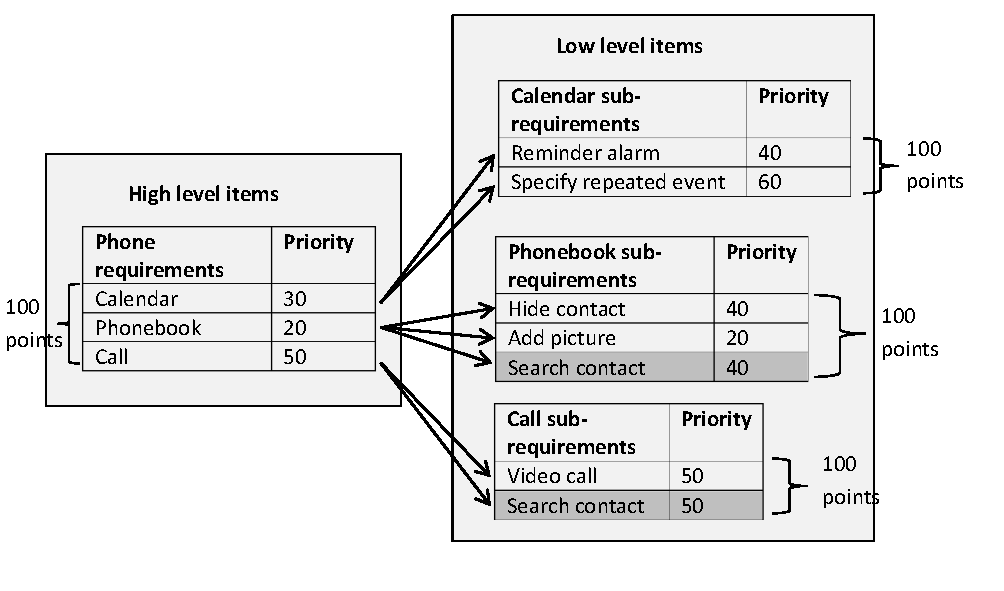
\includegraphics[scale=0.5]{fig/hcv2}

\caption{\label{fig:Example-of-Hierachical}Example of hierarchical cumulative voting with requirement hierarchy.}
\end{figure}

\par\end{flushleft}

\begin{table}
	\scriptsize
\caption{\label{tab:Example-of-Hierarchical}Example of hierarchical cumulative voting.}

\begin{tabular}{
>{\raggedright}p{0.18\columnwidth}
>{\raggedright}p{0.19\columnwidth}
>{\raggedright}p{0.22\columnwidth}
>{\raggedleft}p{0.15\columnwidth}
>{\raggedright}p{0.1\columnwidth}
}
\hline
Phone requirements & Compensation factor & Sub-requirements & Priority calculation & Final priority\tabularnewline
\hline\hline
Calendar & 2 & Reminder alarm & 40{*}30{*}2 & 2400\tabularnewline %\hline
Calendar & 2 & Specify repeated event & 60{*}30{*}2 & 3600\tabularnewline  %\hline
Phonebook & 3 & Hide contact & 40{*}20{*}3 & 1600\tabularnewline %\hline
Phonebook & 3 & Add picture & 20{*}20{*}3 & 800\tabularnewline %\hline
Phonebook \& Call & 3 \& 2 & Search contact & 40{*}20{*}3 + 50{*}50{*}2 & 7400\tabularnewline %\hline
Call & 2 & Video call & 50 {*} 50 {*} 2 & 2500\tabularnewline
\hline
\end{tabular}
\end{table}

